\chapter{Product Taxonomy Matching Methods}
\label{ch:taxonomy-matching}

This Chapter focuses on methods to produce matches in taxonomies and we will describe concrete implementations.
The focus lies on three subcategories of algorithms.
We start with very simple ones that we can use as baselines in our experiments, then move on to
unsupervised algorithms that use external knowledge, like WordNet\footnote{\url{https://wordnet.princeton.edu}. Accessed: 01.05.2020},
and, finally, describe supervised learning algorithms.
They are trained on our dataset and then make predictions on previously unseen pairs.

The goal of each method is to assign a label to a pair of two classes that indicates if they are
equal to each other, if one contains the other, or if they are disjoint, i.e., describing a disjunct set
of entities.

In our implementation, all methods are implemented as normalized similarity measures instead of distances, i.e.,
the results are in a range between 0 and 1 and very similar class-labels are closer to 1.
A distance is 0 when the two inputs match and increases when their similarity decreases.

\section{Baseline Methods}
\label{sec:baseline}

In this Section, we will present simple models that mostly work on the raw category string.
We start with the Levenshtein- or Edit-similarity, move on to the N-Gram-similarity and conclude with
a Path Distance (PD) measure that extends the Levenshtein- and N-Gram-similarity to hierarchies.

\subsection{Levenshtein- or Edit-Similarity}
\label{subsec:levenshtein}

The Levenshtein- or Edit-distance is a simple way to measure the distance between two strings.
It supports a specific set of mutations, and the distance is the number of mutations to get from one
input to another.
The allowed operations are substitution, addition, and deletion of individual characters~\cite{levenshtein1966binary}.
Let us compute the distance between "rose" and "close".
First, we can replace the "r" with an "l" to arrive at "lose" and then add a "c" to the left.
The edit distance between "rose" and "close" is, therefore, two.

Since the edit distance is highly dependent on the length of the word, we use a normalized
distance where we subtract the number of edits divided by the longer string from one.
This subtraction result converts the distance measure into a similarity.
\begin{equation*}
Levenshtein_{sim}(s_1, s_2) = 1 - \frac{Levenshtein_{dist}(s_1, s_2)}{\mbox{max}(\mbox{len}(s_1), \mbox{len}(s_2))}
\end{equation*}
We will use the term Levenshtein-similarity from now on to describe this method.
The Levenshtein-similarity returns a result between 0 and 1, with 0 meaning that there is no relation at all
and 1 meaning that the two strings are the same.

We test multiple thresholds of similarity values on a training dataset and select the best-performing threshold for the final
prediction.
At this point, we need to integrate another trick since we not only want to predict similarity,
but also if one category contains the other or vice versa.
We will apply this trick to all coming measures that only provide a similarity and point to this explanation for reference.

To predict the label, we compute multiple distances.
Obviously, we predict one label between the two unaltered class-labels, but, additionally, we remove the lowest category
in the left and right class-label and compare it with the unaltered right and left class-label.
If such a redacted label is closer to the other class-label, we predict containment instead of equality.
Of those three scores, we take the maximum and, if it exceeds the similarity threshold, we use it to label the category pair.

The following example will illustrate this.
Assume that we want to compare "Clothing, Shoes \& Jewelry $>$ Women $>$ Watches $>$ Smartwatches" with
"Wearable Technology $>$ Smartwatches \& Accessories $>$ All Smartwatches".
We compute the following edit distances:
\begin{itemize}
    \item "Clothing, Shoes \& Jewelry $>$ Women $>$ Watches $>$ Smartwatches" with "Wearable Technology $>$ Smartwatches \& Accessories $>$ All Smartwatches"
    \item "Clothing, Shoes \& Jewelry $>$ Women $>$ Watches" with "Wearable Technology $>$ Smartwatches \& Accessories $>$ All Smartwatches"
    \item "Clothing, Shoes \& Jewelry $>$ Women $>$ Watches $>$ Smartwatches" with "Wearable Technology $>$ Smartwatches \& Accessories"
\end{itemize}
This results in the following tuple of predictions: (0.34, 0.28, 0.3).
In the example above, the Levenshtein-similarity would assign the label \emph{equal} if the threshold is exceeded.

\subsection{N-Gram-Similarity}
\label{subsec:ngram}

This Subsection describes the N-Gram-similarity.
Similar to the Levenshtein-similarity, it only compares the string without any background knowledge about the
hierarchical structure of the input categories.

Euzenat and Shvaiko describe the N-Gram-similarity as follows:
"The n-gram similarity is often used in comparing strings.
It computes the number of common n-grams, i.e.,, strings of n characters, between them.
For instance, trigrams for the string "article" are "art", "rti", "tic", "icl", "cle"."~\cite[p. 90]{euzenat2007ontology}
The formula for the normalized N-Gram-similarity is given as:
\begin{equation*}
    \bar{\sigma}(s, t) = \frac{|ngram(s, n) \cap ngram(t, n)|}{\mbox{min}(|s|, |t|) - n + 1}
\end{equation*}

Again, we test multiple thresholds for the similarity and, since we have another parameter n, also
multiple values for n and select the best parameter combination on the training set.

To predict not only equality, but also \emph{contains} and \emph{contained-in}, we follow the same procedure as already
described in Subsection~\ref{subsec:levenshtein}.

We conclude the N-Gram description by giving an example of how the similarity works.
We compare "Clothing, Shoes \& Jewelry $>$ Women $>$ Watches $>$ Smartwatches" with
"Wearable Technology $>$ Smartwatches \& Accessories $>$ All Smartwatches" with $n = 3$.
Splitting the first string into trigrams results in the following set:
\begin{verbatim}
{('e', 's', ' '), ('J', 'e', 'w'), ('o', 'm', 'e'), ('h', 'e', 's'),
('a', 'r', 't'), ('c', 'h', 'e'), ('m', 'a', 'r'), (' ', 'S', 'h'),
('C', 'l', 'o'), ('o', 'e', 's'), (' ', '>', ' '), ('h', 'i', 'n'),
('n', ' ', '>'), ('h', 'o', 'e'), ('w', 'e', 'l'), ('e', 'n', ' '),
('l', 'o', 't'), (',', ' ', 'S'), (' ', '&', ' '), ('r', 't', 'w'),
('i', 'n', 'g'), ('s', ' ', '&'), ('>', ' ', 'W'), ('s', ' ', '>'),
('t', 'h', 'i'), ('e', 'w', 'e'), ('y', ' ', '>'), ('&', ' ', 'J'),
('r', 'y', ' '), ('S', 'm', 'a'), ('l', 'r', 'y'), ('>', ' ', 'S'),
('m', 'e', 'n'), (' ', 'W', 'a'), ('g', ',', ' '), ('o', 't', 'h'),
('t', 'c', 'h'), ('w', 'a', 't'), ('W', 'a', 't'), ('S', 'h', 'o'),
('t', 'w', 'a'), ('W', 'o', 'm'), ('a', 't', 'c'), (' ', 'W', 'o'),
(' ', 'J', 'e'), ('n', 'g', ','), ('e', 'l', 'r'), (' ', 'S', 'm')}
\end{verbatim}
We carry out the same for the second class and compute the number of intersecting
trigrams for both sets.
We plug this into the nominator of the formula above, calculate the denominator
and arrive at a similarity of $0.321$ for the two strings.

\subsection{Path Similarity}
\label{subsec:path-similarity}

The two baselines methods that we described previously take the full string into account without considering
the hierarchical structure of it.
We introduce a measure that extends those methods to hierarchical strings in this Subsection.

Classes at the top of a hierarchy are, per definition, broader than classes at the lower levels.
In case we want to check if two classes contain the same products, the lower levels are, therefore, more
relevant to our computation.

The path similarity takes this into account and puts high weight on the comparison of the last elements while
reducing the importance of the remainder.
It is derived from the path distance given in~\cite[p. 95]{euzenat2007ontology}, but we implemented it using
similarities.
We define path similarity as:
\begin{equation*}
    \sigma(s^n, t^m) = \lambda \cdot \hat{\sigma}(s^n, t^m) + (1 - \lambda) \cdot \sigma(s^{(n-1)}, t^{(m-1)})
\end{equation*}
where $s^n$ and $t^m$ are sequences of strings and $\hat{\sigma}$ is a string-based similarity function, like one of
those introduced in Subsection~\ref{subsec:levenshtein} and~\ref{subsec:ngram}.
If one sequence is empty, $\sigma$ returns 0 as the similarity.

Again, we apply the similarity function to "Clothing, Shoes \& Jewelry $>$ Women $>$ Watches $>$ Smartwatches" with
"Wearable Technology $>$ Smartwatches \& Accessories $>$ All Smartwatches" and use the Levenshtein-similarity internally.
We assume that $\lambda = 0.7$.
First, we compare "Smartwatches" with "All Smartwatches" with the Levenshtein-similarity and multiply this with $\lambda$.
This results in an intermediary result of 0.525.
Next, we call the path-similarity recursively with the remainder, i.e., "Clothing, Shoes \& Jewelry $>$ Women $>$ Watches"
and "Wearable Technology $>$ Smartwatches \& Accessories".
The result is multiplied with 0.3 and added to the already computed 0.525.
In the last recursive call, we compare "Clothing, Shoes \& Jewelry" with nothing and, in this case, simply return 0.

The overall similarity between our input strings is 0.583.
In our experiments, we will use the Levenshtein- and N-Gram-similarity for $\hat{\sigma}$.

In this Section, we introduced three baseline methods that use simple string similarity measures and one that
uses the hierarchical structure to compute a similarity between two classes.
They will serve as a baseline to compare the more advanced algorithms to, which we will present in the coming
sections.

\section{WordNet-Based Matching Methods}
\label{sec:unsupervised-taxo-match}

This Section covers unsupervised taxonomy matching methods, i.e., methods that take as input the raw classes
and other static third-party resources like WordNet~\cite{miller1995wordnet}.
We only use the training dataset to optimize certain hyperparameters.
First, we introduce S-Match or Semantic Match~\cite{giunchiglia2005semantic}, which is a generic taxonomy
mapping algorithm that provides semantic annotations, i.e., not only \emph{equal} or best-match predictions,
but also labels for \emph{contains}, \emph{contained-in}, and \emph{disjoint} relations.
The second algorithm is an extension of the product taxonomy mapping algorithm by Park and Kim~\cite{park2007ontology}
and is called SCHEMA~\cite{aanen2012schema}.

\subsection{S-Match}
\label{subsec:smatch}

Giunchiglia et al.\@~\cite{giunchiglia2005semantic} state that S-Match is based on two fundamental ideas:
\begin{itemize}
    \item Discover mappings by computing semantic relations.
    \item Determine semantic relations by analyzing the meaning.
\end{itemize}
Contrary to the approaches we described earlier, there is no threshold or hyperparameter that we can tune.
Instead of computing a similarity, the algorithm translates the taxonomies into a satisfiability problem
and computes a relation directly.

The authors use specific terms to identify parts of the taxonomy.
We will first introduce the terms and then describe the individual steps of the algorithm.
A taxonomy is a tree-like structure and consists of \emph{labels} and \emph{nodes}.
Labels are individual edges in the tree, e.g.,
"Clothing, Shoes \& Jewelry $>$ Women $>$ Watches $>$ Smartwatches" contains the labels
"Women", "Watches", etc.
The whole string is called a node.
In our case "node" translates to "class-label" and "label" to "category".
We will continue the explanation using our terms.

S-Match has four steps that are used to match two taxonomies:
\begin{enumerate}
    \item Compute the concepts of all categories in the tree.
    \item Compute the concepts of all class-labels in the tree.
    \item Compute relation between all concepts of category-pairs.
    \item Compute relation between all concepts of class-label pairs.
\end{enumerate}

Step 1 takes each category, e.g., "Watches", and computes the meaning of the category.
To extract the meaning, S-Match relies on an external source or oracle, in this case, WordNet.
Instead of using "Clothing, Shoes \& Jewelry" directly, the terms are first split up
(tokenized), then reduced to a normalized form (stemmed) and then mapped to one
or more WordNet senses.
The provided example would result in "Clothing | Shoes | Jewelry" $\Rightarrow$ "Cloth | Shoe | Jewelry"
$\Rightarrow$ "cloth.n.01 | shoe.n.01 | jewelry.n.01".
In the case of multiple terms, we take the logical disjunction of them and use it as the concept of the category.
The concept of the category "Clothing, Shoes \& Jewelry" would, therefore, be "cloth.n.0.1 $\vee$ shoe.n.01 $\vee$ jewelry.n.01".

The next step combines the concept of all categories in a class-label into the concept of a class-label.
We use the conjunction of category concepts, which would result in the following logical formula for our example:
"(cloth.n.0.1 $\vee$ shoe.n.01 $\vee$ jewelry.n.01) $\wedge$ (women.n.01) $\wedge$ (watch.n.01) $\wedge$ (smartwach.n.01)".

All of the steps above only rely on information present in a single taxonomy and the corresponding oracle.
Hence, we can consider them as "offline" since they can be precomputed.
The last two steps combine information from multiple taxonomies and are, therefore, considered to be "online".

In the third step, we build up a relation matrix between the concepts of categories.
Every category in the one taxonomy is matched with every category from the other taxonomy using a group of matchers.
\begin{figure}[!htbp]
    \centering
    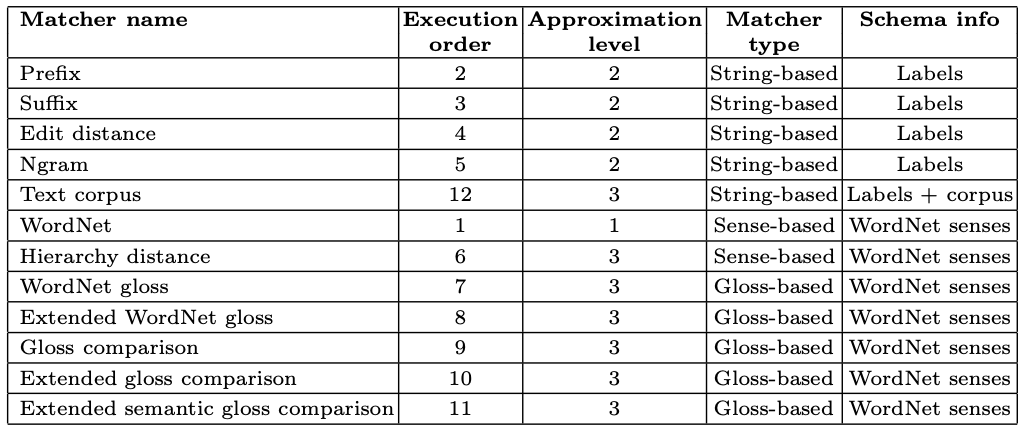
\includegraphics[width=13cm]{images/smatch-matchers.png}
    \caption[S-Match Matching Methods]{S-Match Matching Methods\protect~\cite{giunchiglia2005semantic}}
    \label{fig:smatch-matchers}
\end{figure}

As we can see in Figure~\ref{fig:smatch-matchers} the matchers are categorized into three approximation levels.
The first level relies strictly on the WordNet meaning computed in step 1 and relations returned by it are always correct.
In case a matcher on one level does not provide a confident prediction, there is an automatic fallback to the next method and level.
The second approximation level relies mostly on the actual strings of the category.
String-based methods like the Levenshtein-similarity are used, and in case they are unable to provide a relation
additional, but more unreliable, features of WordNet are applied.
Some of those are inspired by COMA++ by Aumueller et al.\@~\cite{aumueller2005schema}.

Now, that the category relations are available, we can match class-labels.
To do this, we will compare the class-label already given above with "Jewelry \& Watches $>$ Watches, Parts \& Accessories".
S-Match predicts a relation between the first two categories in both nodes, but is not sure which relations holds.
It gives a firm prediction that "Watches" is contained-in "Watches, Parts \& Accessories".
This is translated into a satisfiability problem of the form $axiom \rightarrow rel(concept_l, concept_r)$
where $rel$ is the relation we want to prove.
In this case, we will simply try the \emph{contained-in} relation, formulate the negation $axiom \wedge \lnot rel(concept_l, concept_r)$.
At this point in time, DPLL~\cite{davis1962machine} is used to check for satisfiability, and if it finds a contradiction,
we predict the given relation.

The authors provide an implementation that is hosted on GitHub\footnote{\url{https://github.com/opendatatrentino/s-match}. Accessed: 01.05.2020},
which we will reuse for our experiments.

\subsection{SCHEMA}
\label{subsec:schema}

The second algorithm in this Section is SCHEMA by Aanen et al.\@~\cite{aanen2012schema}.
It extends on the ideas of Park and Kim~\cite{park2007ontology} in the sense that they also use
word sense disambiguation on top of WordNet~\cite{miller1995wordnet}.
Since SCHEMA is supposed to be a mapping algorithm that simply finds the best-match between two nodes
in a taxonomy, we deviate slightly from the algorithm described by Aanen et al.
The algorithm also provides a semantic match in the sense that it compares a source and a target node
and predicts if the source node contains the target node.
To map this to our desired outputs, we take each node as a source \emph{and} as a target node.
If they are both labelled as supersets of each other, we predict \emph{equal}.
If only one is a superset of the other,
we label it as \emph{contains}, and if none of the above conditions apply, we label the pair as \emph{disjoint}.

SCHEMA is implemented in three steps:
\begin{enumerate}
    \item Source Category Disambiguation.
    \item Candidate Target Category Selection.
    \item Candidate Target Path Key Comparison.
\end{enumerate}
The first step takes the source category and tries to find its intended meaning.
Composite classes frequently occur in product taxonomies.
We already saw an example in the previous Section: "Clothing, Shoes \& Jewelry".
All of those could be a class in itself and may lead to problems, since another online shop may
combine their products in different composite classes.
Hence, they are separated into a split-term set.

Now, the sense for every split-term is computed.
The authors propose to use WordNet to get synonyms of the current term and, to exclude misleading senses,
use the terms in the parent element of the hierarchy to provide a context to filter the synonyms.
Taking "Watches $>$ Bands" as an example, we would take "Bands" as the split term set and compute its synonyms.
Now, it might be possible that a "Band" in terms of a music-making group is included there.
SCHEMA also adds the context of "Watches" into this consideration and, therefore, the music-making group
can be excluded, while the sense of a watch-band is retained.
The foundation of this idea is taken from Lesk~\cite{lesk1986automatic}.

Given the senses and synonyms of the source category, close categories in the target taxonomy can be found.
For each pair of categories, a semantic match is computed that labels the target category as containing the
source category or the two categories as \emph{disjoint}.
Similar to S-Match~\ref{subsec:smatch} there are multiple matchers used in this prediction.
The target category contains the source category, if the senses of the source category are a subset of it, e.g.,
"Shoe" as the source category would be contained-in "Clothing, Shoes \& Jewelry".
If this is ambiguous, the Levenshtein-similarity is applied, and if it exceeds a given threshold,
the source category is also labelled as being a subset of the target category.

Out of the target categories that contain the source relation, SCHEMA would try to find the best match in the third
step to create a mapping between them.
Since we want to compare two categories directly, we skip the third step and, instead, switch source and target categories
and run the prediction again.
This results in an \emph{equal}, \emph{contains}, \emph{contained-in} or \emph{disjoint} prediction.

Our implementation is based on an open-source implementation of SCHEMA with a few extensions to our use case.
See GitHub\footnote{\url{https://github.com/nudge/schema}. Accessed: 01.05.2020} for the reference implementation.

\section{Supervised Taxonomy Matching Methods}
\label{sec:supervised-taxo-match}

One of the major drawbacks of the WordNet-based taxonomy matching methods is that the WordNet corpus
is kind of small compared to the number of possible words that may be used in taxonomies across the web.
If the word is out of the given vocabulary, no synonyms and, therefore, no similarity can be computed.

We propose multiple methods in the following Section that introduce certain ways to avoid this limitation
of WordNet-based models.

At first, we will have a look at word embedding based models following Zhang et al.\@~\cite{zhang2014ontology}.
Then, we use standard Python libraries to derive features from the given classes and apply
machine learning classification algorithms.

\subsection{Ontology Matching with Word Embeddings}
\label{subsec:word-embeddings}

Zhang et al.\@~\cite{zhang2014ontology} claim that the WordNet corpus is insufficient for taxonomy matching and
propose to use word embeddings instead.
They use word2vec~\cite{mikolov2013distributed} on the Wikipedia corpus to compute an embedding of each word
and apply the Cosine similarity (CS) to calculate the similarity between words.
For each entity in one taxonomy, they find the most similar entity in the other taxonomy given the entity's embedding.

While word embeddings are able to greatly enhance the available vocabulary, they may introduce new problems,
since they tend to coalesce semantic similarity and conceptual association.
"Horse" and "Harness" may be similar and in a related context, but they should not be matched in
a taxonomy matching task~\cite{kolyvakis2018deepalignment}.

Since Zhang et al.\@ only try to find the most similar class
and we intend to classify a pair of classes, we use a slightly different setup.
We employ a pre-trained word2vec model trained on about 100 billion Google news word that can be downloaded
via Gensim~\cite{rehurek2010gensim}.
For every word in a class, we retrieve its embedding, a 300-dimensional vector, and take an average of the
individual word vectors to represent the whole class.
Afterwards, we compute the similarity for both complete class-labels and with the lowest category removed on each class as
as performed in Section~\ref{subsec:levenshtein} and~\ref{subsec:ngram}.

We use those similarity scores to make a prediction.
If a word is still not included in our vocabulary, we simply ignore it.
A possible future extension may be the usage of fastText\footnote{\url{https://fasttext.cc}. Accessed: 01.05.2020}
that also enables the embedding of out-of-vocabulary words.
Another extension could be an increased weight of the lower-level labels in the class hierarchy.

\subsection{Machine Learning Classification}
\label{subsec:machine-learning}

The problem we cover in this Thesis is finding the most suitable label for a pair of classes that
come from e-commerce product taxonomies.
This can be reduced to a standard machine learning classification, where two inputs are given
and an output label should be predicted.
We, therefore, deviate from the approaches of the ontology matching literature and focus on
standard machine learning classification algorithms as provided by scikit-learn\footnote{\url{https://scikit-learn.org/stable/index.html}. Accessed: 01.05.2020}.

To apply the machine learning algorithms, we have to transform our class strings into a numeric vector that
can be fed into the models.
We use the included CountVectorizer\footnote{\url{https://scikit-learn.org/stable/modules/generated/sklearn.feature\_extraction.text.CountVectorizer.html}. Accessed: 01.05.2020},
which indicates basically how often a certain word appears in the given string.
We also use the word2vec model to compare the results of both embedding models.

Imagine a dataset of the following strings:
\begin{itemize}
    \item One Ring to rule them all, One Ring to find them,
    \item One Ring to bring them all and in the darkness bind them.
\end{itemize}
If we reduce our vocabulary to the strings [one, ring, rule, them, all, find, darkness, bind, bring]
the two sentences result in the following vectors:
\begin{itemize}
    \item $[2, 2, 1, 2, 1, 1, 0, 0, 0]$
    \item $[1, 1, 0, 2, 1, 0, 1, 1, 1]$
\end{itemize}
Since product taxonomies are structured, they do not contain any stop word that should usually be removed.
We also expect words to be normally distributed and, therefore, do not weight the results by inverse document
frequency (c.f.\@ tf-idf).
The resulting vector has a number of dimensions  that is equal to the vocabulary size.
Next, the input dataset is transformed by replacing the strings with vectors and concatenating the
two vectors to produce a single feature vector.

For the prediction, we considered the following classification models.
We started with multinomial Naive Bayes, "one of the two classic naive Bayes variants used in text
classification"\footnote{\url{https://scikit-learn.org/stable/modules/naive_bayes.html#multinomial-naive-bayes}. Accessed: 01.05.2020}.
Based on the training data, a distribution is parameterized that predicts the probability of a label, given the
evidence.

The next algorithm is Stochastic Gradient Descent (SGD)\footnote{\url{https://scikit-learn.org/stable/modules/linear_model.html#stochastic-gradient-descent-sgd}. Accessed: 01.05.2020},
which trains a linear classifier (Support Vector Machine (SVM)/Logistic Regression) depending on the provided loss function.
In our case, the optimal loss function is derived via the grid search.
A linear classifier aims to find a decision boundary or hyperplane that separates differently labelled points in the
vector space and makes predictions based on this hyperplane.

We also use AdaBoost\footnote{\url{https://scikit-learn.org/stable/modules/generated/sklearn.ensemble.AdaBoostClassifier.html}. Accessed: 01.05.2020},
an ensemble method that combines multiple classifiers to enhance its predictions.
It relies on simple decision trees and, after finding a good initial fit, it trains additional models with different
parameters to optimize for edge cases.

Finally, we train a Multi-Layer Perceptron (MLP)\footnote{\url{https://scikit-learn.org/stable/modules/generated/sklearn.neural_network.MLPClassifier.html}. Accessed: 01.05.2020},
a kind of Neural Network.
It combines multiple layers of neurons that use a non-linear activation function and is trained similarly to the SGD
models.
Sonoda and Murata~\cite{sonoda2017neural} show that a Neural Network with sufficient neurons is a universal approximator,
i.e., it can represent any function arbitrarily well.
Hence, with sufficient training data and a sufficiently complex model, we can represent the training data perfectly.
Given the limited size of our gold standard, we will use simple Neural Network models in our evaluation.

To optimize the hyperparameters of the machine learning models, we use grid search, i.e., different hyperparameters
are tested on a subset of the actual training data and the final model is trained using the optimal hyperparameters and
the full training set.
In Table~\ref{tab:grid-search} we present the parameters that were tested for each model described above.
We will only list the parameters in which we deviated from the default or, in case the default is among the possible values,
highlight it in bold.
For a description of the individual model parameters, we refer the reader to the excellent scikit-learn documentation
referenced in the footnote of the specific model.

\begin{table}[htbp]
    \begin{center}
        \begin{tabular}{l|l|l}
            Model              & Parameter            & Values \\
            \hline
            SGDClassier        & alpha                & 0.01, 0.001 \\
                               & loss                 & \textbf{hinge}, modified\_huber \\
            AdaBoostClassifier & learning\_rate       & 0.3, \textbf{1.0}, 1.7 \\
                               & algorithm            & SAMME, \textbf{SAMME.R} \\
            MLPClassifier      & activation           & logistic, \textbf{relu} \\
                               & hidden\_layer\_sizes & (50,), (25, 25), (50, 25) \\
                               & alpha                & \textbf{0.0001}, 0.0003, 0.001 \\
        \end{tabular}
        \caption{Grid Search Hyperparameters.}
        \label{tab:grid-search}
    \end{center}
\end{table}

\section{Summary}

In this Chapter, we introduced multiple classification methods for class-label pairs derived from e-commerce taxonomies.
We used naive string matching methods as a baseline and an enhanced version that takes the hierarchical structure into account.
Two suitable algorithms from related literature were introduced that use WordNet as an oracle for providing synonyms.
Finally, a method based on current research using word embeddings to circumvent WordNet's limitations and
an ensemble of open source machine learning classification methods were employed.

%Idea: Use standard similarity measures and combine their output using a machine learning
%classifier~\cite{nezhadi2011ontology, nkisi2018ontology, eckert2009improving}.
%Eckert et al.\@ show that not only the raw matcher outputs should be  added to the ML phase,
%but also meta information about the taxonomy.
%This enables to algorithm to determine how much he can trust an individual matcher.
%Foundation of their idea is combining classifiers~\cite{kittler1998combining}.
